\section{Work So Far}

\begin{frame}{Work So Far}
	Thus far, most of the work on my thesis has been split between three tasks:
	
	\begin{enumerate}
		\item Familiarising with one particular implementation: JIF (Java Information Flow)
		\item Researching information flow models and implementations
		\item Researching the applicability of information flow to real security problems
	\end{enumerate}
\end{frame}

\begin{frame}{JIF}
	Java Information Flow is a language extension to Java with `mostly static' information flow features through the addition of `security types', with policies as per the Decentralised Label Model \cite{work:myersdlm}.
	
	Every variable has a security label attached to it which encodes how its information may flow between principals. For instance:
	
	\texttt{int\{Alice->Bob\} x;}
	
	indicates that principal Alice owns the information, and allows that information to flow to Bob or a principal Bob has delegated authority to. A third principal, Charlie, would not be allowed to access this information.
\end{frame}

\begin{frame}{JIF: Static Checking Errors}
	\begin{figure}
		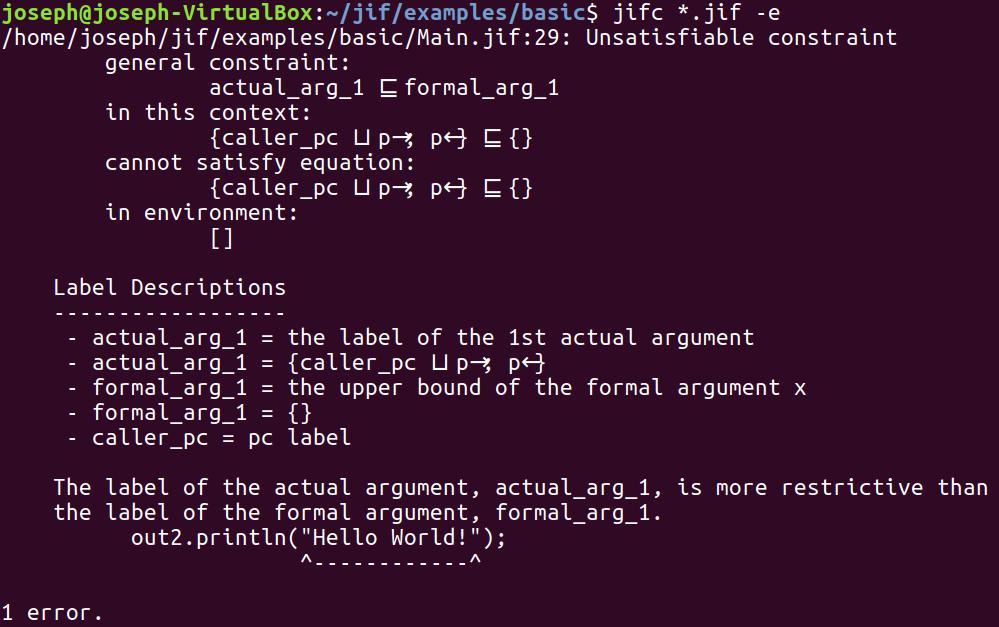
\includegraphics[scale=0.5]{content/images/jif_helloworld_error.png}
		\caption{A JIF compiler error}
	\end{figure}
\end{frame}

\begin{frame}{JIF: A Minimal `Hello World'}
	\begin{figure}
		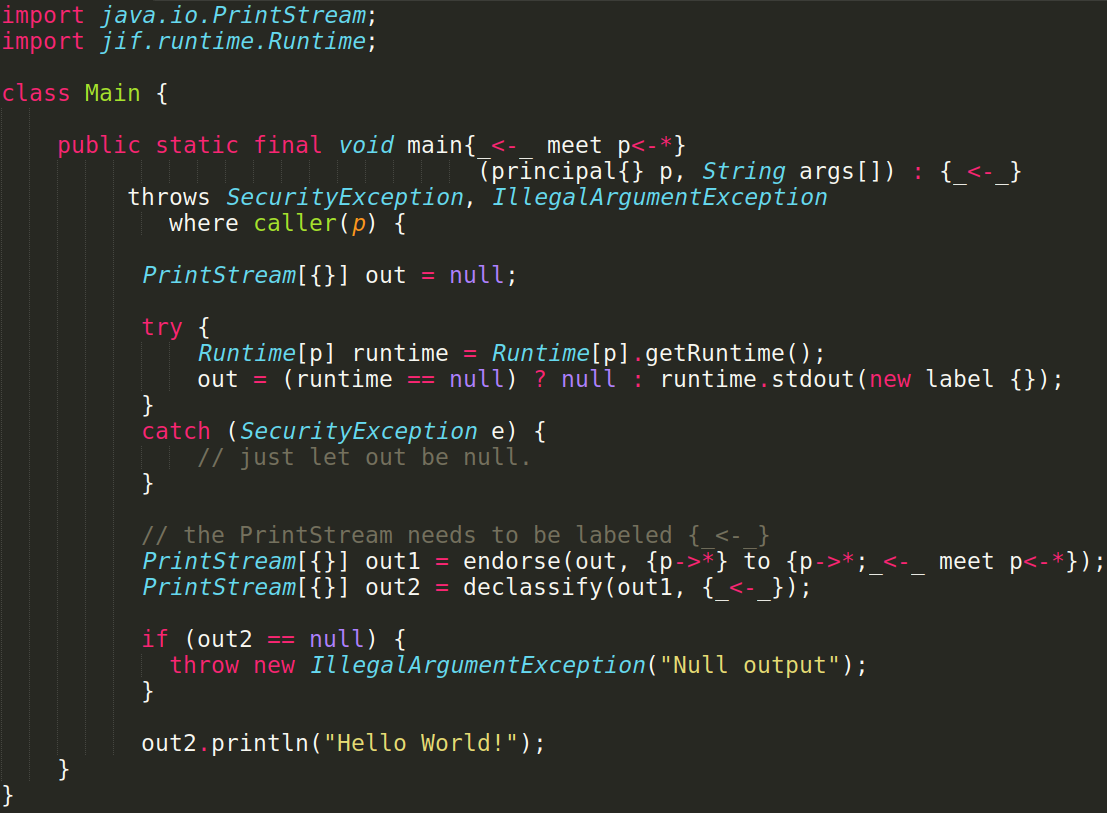
\includegraphics[width=\linewidth]{content/images/jif_helloworld.png}
	\end{figure}
\end{frame}

\begin{frame}{JIF: Practicality \& Programmer Burden}
	Content...
\end{frame}

\begin{frame}{Other Implementations}
	\begin{enumerate}
		\item Paragon
		\item LIFTy
	\end{enumerate}
\end{frame}

\begin{frame}{General Applicability}
	Oracle Guidelines
	
	Untrusted code vs Untrusted data
	
	Actual exploits
\end{frame}

\begin{frame}{Overall Thoughts}
	`Heavy' programmer burden
	
	Not relevant for most security issues
\end{frame}